\documentclass[compress,]{beamer}

%presentation layout

\mode<presentation>
{
  \usetheme{Berlin}
  % \usecolortheme{dove}
  \setbeamercolor{structure}{bg=black,fg=white}
  \setbeamercolor{normal text}{bg=black,fg=white}
  \setbeamercolor{titlepage}{bg=black,fg=white}
  \setbeamercolor{titlelike}{bg=black,fg=white}
  \setbeamercolor{palette primary}{bg=black}
  \setbeamercolor{palette secondary}{bg=black, fg=gray}
  \setbeamercolor{palette tertiary}{bg=black, fg=gray}
  \setbeamercolor{palette quarternary}{bg=black}
  \setbeamercovered{transparent}
  \useinnertheme{rectangles}
  %\usefonttheme{serif}
}

\setbeamertemplate{navigation symbols}{}

%loading packages
\usepackage[ngerman]{babel}
\usepackage[T1]{fontenc}
\usepackage[utf8]{inputenc}
\usepackage{graphicx}
\usepackage{amsmath}

% vorgeplaenkel
\title[ZäPFchen-Einführung]{ZäPFchen-Einführung}

\author{Ständiger Ausschuss aller Physikfachschaften}

\institute[Zusammenkunft aller Physikfachschaften]

\date{\today}

\subject{ZäPFchen-Einführung}

\begin{document}

\begin{frame}
  \titlepage

  % \begin{figure}
  %   \centering
  %   \includegraphics[]{}
  % \end{figure}
\end{frame}

\section{ZäPFchen-Einführung}

%%%Folie 1

\section{ZaPF?}

\begin{frame}{Warum sind wir überhaupt hier?}

  \begin{itemize}
  \item Physik-Fachschaften vernetzen
  \item Diskussion
  \item Probleme lösen
  \item Positionen erarbeiten
  \end{itemize}

\end{frame}

%%%Folie 2

\section{Was passiert mit mir?}

\subsection{Ablauf}

\begin{frame}{Ablauf}

  \begin{figure}
    \centering
    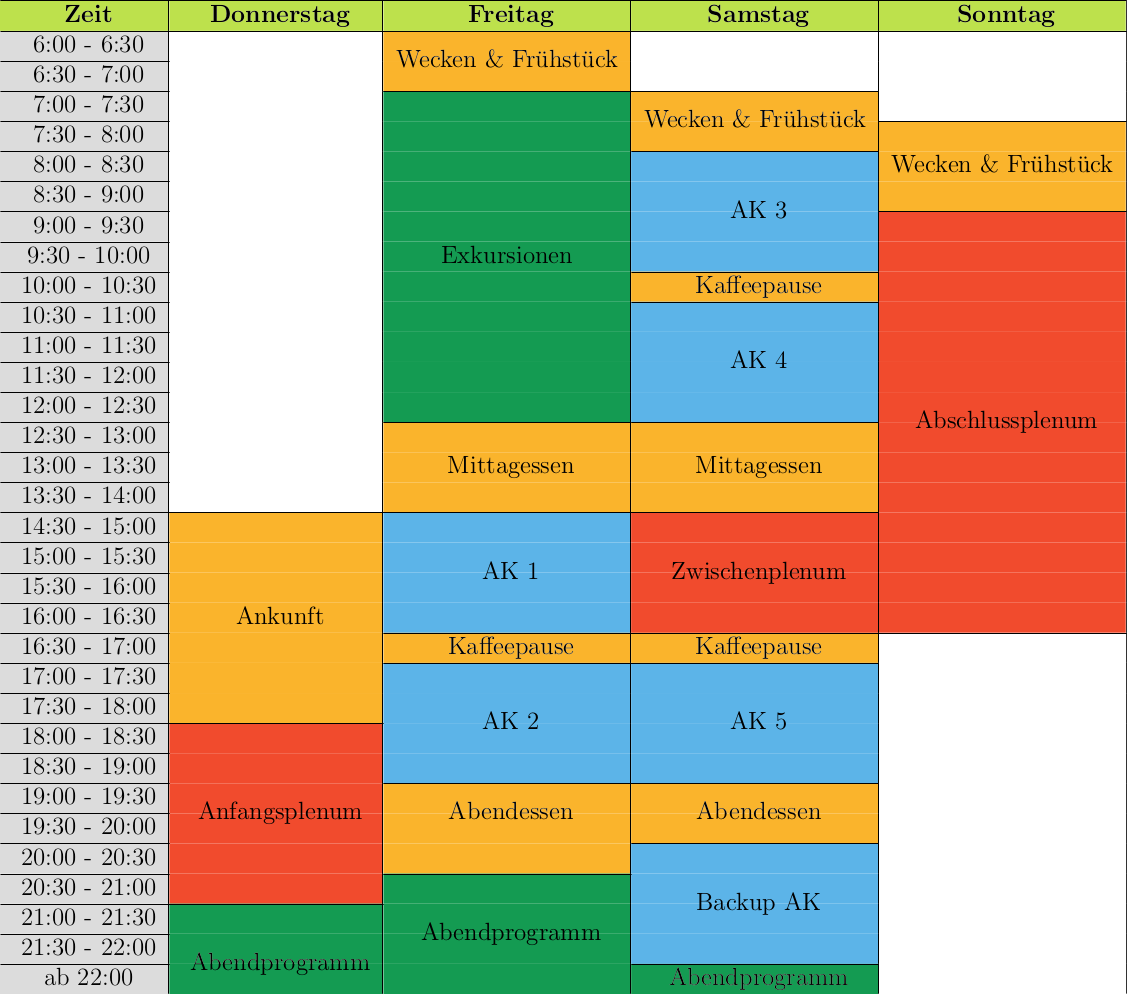
\includegraphics[scale=0.35]{./fig/ablaufplan_frankfurt_wise2015}

    \caption{Also kurz: Essen, Plenum, AKe und Spaß}
  \end{figure}

\end{frame}

%%%Folie 3

\subsection{Aufbau}

\begin{frame}{Plenum? Plenums? Plena?}

  \begin{itemize}[<+->]
  \item \textbf{Was ist es?} Das oberste beschlussfähige Gremium der ZaPF.
  \item \textbf{Wer?} Das ZaPF-Plenum sind wir alle gemeinsam.
  \item \textbf{Wann?} Anfang und Ende und dazwischen auch.
  \item \textbf{Was passiert?} Wahlen, Abstimmungen, Vorstellen von Ergebnissen

    Ergebnisse kommen aus Arbeitskreisen, die im Anfangsplenum eingeteilt werden.
  \end{itemize}

%%%Folien 4

\end{frame}

\begin{frame}{Was ist ein Arbeitskreis?}

  \begin{itemize}[<+->]
  \item Wieso? Im Plenum diskutieren ist anstrengend.

    In kleine(re)n Gruppen zu sprechen ist effektiv und zeitsparend
  \item Wann? Zweistündige Slots an allen Tagen außer am ersten und letzten.
  \item Wie? 5 bis 30 Teilnehmer

    Teilweise mit Gästen, Vorträge, Workshops oder andere Formate
  \item Arten?
    \begin{itemize}[<+->]
    \item ``Normal'': Diskussionen und Austausch
    \item Austausch-AK: viele kurze Themen
    \item Folge-AK: braucht meist Vorwissen
    \item Spaß-AKs (Ausnahmen): Bier-Austausch, Fachschaftsfreundschaften
    \end{itemize}
  \end{itemize}

\end{frame}

%%%Folie 5

\section{Materialien}

\subsection{GO}

\begin{frame}{GO, GO, Geschäftsordnung!}

  \begin{itemize}[<+->]
  \item<1-> \textbf{Warum brauchen wir das?} Plenen können aus dem Ruder
    laufen.

    Die GO kann das wieder einfangen.
  \item<2-> \textbf{Wo zu finden?} Im Tagungsheft.
  \item<3-> \textbf{GO-Anträge} (Beide) Hände hoch! In der GO nachlesen.

    \visible<4->{\Huge{Vorher nachdenken.}}
    \begin{itemize}
    \item<5-> Begrenzung der Redezeit
    \item<6-> Schließen der Redeliste
    \item<7-> Unterbrechung
    \item<8-> \ldots
    \end{itemize}
  \item<9-> GO gilt nicht in AKen
  \end{itemize}

\end{frame}

%%%Folie 6

\subsection{Protokolle}

\begin{frame}{Protokolle}

  \begin{itemize}
  \item<1-> Zu jedem AK \emph{muss} ein Protokoll geschrieben werden.
  \item<2-> \textbf{Wie?} Vorlagen sind im Wiki.

    \visible<3->{\Huge{Benutzt sie.}}
  \item<4-> \textbf{Warum?}
    \begin{itemize}
    \item<5-> Weitere Arbeit an selben Themen (Folge-AKs)
    \item<6-> Fasst AKe zusammen
    \item<7-> Füllen Gedächtnislücken
    \end{itemize}
  \item<8-> Werden für die Nachwelt im Reader und im Wiki erhalten
  \end{itemize}

\end{frame}

%%%Folie 7

\subsection{ZaPF-Wiki}

\begin{frame}{Hey¸ hey, Wiki! hey, Wiki, hey!}

  \begin{itemize}[<+->]
  \item ZaPF-Wiki = Arbeitsplattform
  \item Sammelt Ergebnisse von ZaPFen
  \item Bereitet ZaPFen vor
  \item \Huge{ZaPF-Wiki is love!}
  \item \Huge{ZaPF-Wiki is life!}
  \end{itemize}

\end{frame}

\begin{frame}{Benutzerkonto erstellen}
  \centering
  \Huge{Alt + Tab}

\end{frame}

%%% Folie 8

\section{Ihr!}

\begin{frame}{Ihr!}

  Macht was draus.

\end{frame}

\end{document}

%%% Local Variables:
%%% mode: latex
%%% TeX-master: t
%%% End:
